\subsection{Функции высшего порядка}

\begin{frame}
	\tableofcontents[currentsection,currentsubsection]
\end{frame}

\begin{frame}{Напоминание}
	\begin{itemize}
		\item Функция является \textit{функцией высшего порядка}, если она в качестве одного из аргументов принимает другую функцию.
		\item Пример: \t{map}. Он первым параметром принимает функцию, которая преобразует элементы списка.
		\item Пример: \t{dropWhile}. Первый аргумент умеет по элементу сообщать, надо остановиться или нет.
		\item Пример: \t{filter cond list}. Оставляет в списке только элементы, удовлетворяющие условию.
		\item Функции высшего порядка является основными кирпичиками в функциональном программировании.
	\end{itemize}
\end{frame}

\begin{frame}[fragile]{Ещё один паттерн}
\begin{minted}{haskell}
sum (x:xs) = x + sum xs
sum _ = 0

prod (x:xs) = x * prod xs
prod _ = 1

max (x:xs) = max x (max xs)
max x = -1

concat (x:xs) = x ++ (concat xs)
concat _ = ""
\end{minted}
	Что общего?
	\pause
	\begin{itemize}
		\item Все эти функции считают функцию от множества элементов.
		\item Для пересчёта требуется знать только текущее значение и очередной элемент.
	\end{itemize}
\end{frame}

\begin{frame}[t,fragile]{Правая свёртка}
\begin{minted}{haskell}
foldr f a (x:xs) = f x (foldr f a xs)
foldr f a _ = a

sum    xs = foldr (+)  0    xs
prod   xs = foldr (*)  1    xs
max    xs = foldr max  (-1) xs
concat xs = foldr (++) ""   xs
\end{minted}
	Ещё одна популярная функция высшего порядка.
\end{frame}

\begin{frame}[fragile]{Упражнение на понимание}
\begin{minted}{haskell}
foldr f a (x:xs) = f x (foldr f a xs)
foldr f a _ = a
\end{minted}

	А что такое \t{foldr (:) [4,5] xs}?
	\pause
\begin{minted}{haskell}
foldr (:) [4,5] [1,2,3] =
1:(foldr (:) [4,5] [2,3]) =
1:(2:(foldr (:) [4,5] [3])) =
1:(2:(3:(foldr (:) [4,5] []))) =
1:(2:(3:[4,5])) =
[1,2,3,4,5]
\end{minted}
	Дописывание \t{[4,5]} в конец списка.

\begin{minted}{haskell}
(++) a b = foldr (:) b a
\end{minted}
\end{frame}

\begin{frame}{Картинка}
	\begin{center}
		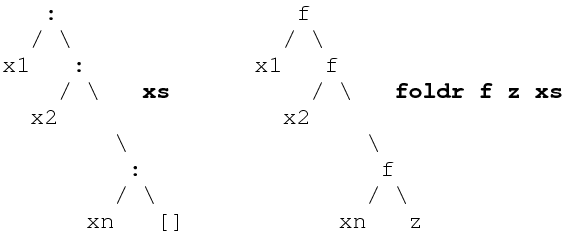
\includegraphics[scale=0.5]{foldr.png}
	\end{center}
	Бамбук растёт вправо, поэтому \textit{правая} свёртка.
\end{frame}

\begin{frame}[fragile]{Упражнения}
	Как узнать, все ли элементы равны \t{True}? \pause
\begin{minted}{haskell}
foldr (&&) True xs
\end{minted}

	Как узнать сумму квадратов чисел в массиве? \pause
\begin{minted}{haskell}
foldr (+) 0 (map (^2) xs)
\end{minted}

	Как выразить \t{map} через \t{foldr}? \pause
\begin{minted}{haskell}
map f xs = foldr (\a x -> (f a):x) [] xs
\end{minted}
	Вывод: в теории почти всё есть \t{foldr}.
	На практике лучше использовать готовые функции.
\end{frame}
